\documentclass[11pt]{article}

% basic packages
\usepackage[margin=1in]{geometry}
\usepackage[pdftex]{graphicx}
\usepackage{amsmath,amssymb,amsthm}
\usepackage{william}
\usepackage{tikz-cd}
\usepackage{extarrows}
\usepackage{changepage}

% page formatting
\usepackage{fancyhdr}
\pagestyle{fancy}

\renewcommand{\sectionmark}[1]{\markright{\textsf{\arabic{section}. #1}}}
\renewcommand{\subsectionmark}[1]{}
\lhead{\textbf{\thepage} \ \ \nouppercase{\rightmark}}
\chead{}
\rhead{}
\lfoot{}
\cfoot{}
\rfoot{}
\setlength{\headheight}{14pt}

\linespread{1.03} % give a little extra room
\setlength{\parindent}{0.2in} % reduce paragraph indent a bit
\setcounter{secnumdepth}{2} % no numbered subsubsections
\setcounter{tocdepth}{2} % no subsubsections in ToC

\begin{document}

% make title page
\thispagestyle{empty}
\bigskip \
\vspace{0.1cm}

\begin{center}
{\fontsize{22}{22} \selectfont Lecture Notes on}
\vskip 16pt
{\fontsize{36}{36} \selectfont \bf \sffamily Groups and Representations}
\vskip 24pt
{\fontsize{18}{18} \selectfont \rmfamily \href{https://will-lancer.github.io}{Will Lancer}} 
\vskip 6pt
{\fontsize{14}{14} \selectfont \ttfamily will.m.lancer@gmail.com} 
\vskip 24pt
\end{center}

{\parindent0pt \baselineskip=15.5pt}
\noin
Notes on group and representations, as used in physics. Resources used:
\begin{itemize}
    \item Peter van Nieuwenhuizen's PHY 680 course at SBU,
    and the lecture notes from the course. This is the primary
    source of content; I just explain things in my own way, and
    make things more formal and precise.
    \item Andre Lukas' 
    \href{https://www-thphys.physics.ox.ac.uk/people/AndreLukas/GroupsandRepresentations/groupsrepslecturenotes.pdf}{lecture notes} 
    on groups and representations.
    \item Fulton and Harris' \emph{Representation Theory: A First Course}.
    \item Georgi's \emph{Lie Algebras in Particle Physics}.
\end{itemize}

% make table of contents
\newpage
\microtoc
\newpage

% main content

\section{Finite Groups and Representations}

We begin by collecting the most important facts about the representation
theory of finite groups. At the end, we touch on Majorana spinors and the normal
modes of atomic molecules. For general background, see the notes on
algebra \href{https://github.com/will-lancer/notes/blob/main/Mathematics/Algebra/Algebra.pdf}{here}.

\subsection{Finite groups}

\begin{eexample}
    [The most important finite groups for physics]
    Of course, the most important groups for physics are (semi-simple)
    Lie groups, but there are a few important finite ones as well:
    \begin{itemize}
        \item $S_n$. This group is good for talking about permutations
        of objects, and is necessary for talking about group actions.
        \item $A_n$. See above, but sometimes we only want even permutations.
        \item $D_n$. Because $D_n$ is, by definition, the group of isometries
        of a planar $n$-point object, this is useful to look at when studing
        planar objects. We can also think about certain continuous groups
        as limits of $D_n$, e.g. emergent $O(N)$ symmetry in spin systems.
        \item $\ints/n\ints$. These groups are useful for a number of things.
        $\ints/2\ints$ is parity, and modding out by it also produces quite
        a few useful Lie groups (e.g. $SU(2)/\ints/2\ints \cong SO(3)$). It also
        catalogues cyclic groups, so it's useful when we want to think about
        those ideas. Additionally, these groups are closely connected to number
        theory when $n = p$ is prime, and there are more and more connections
        between physics and number theory as time goes on$\ldots$
    \end{itemize}
\end{eexample}

We now get into the most important definitions behind finite
group theory for physics.

\begin{definition}
    Consider $\gamma_g \colon G \to G$ by $\gamma_g(a) = g a g^{-1}$.
    We say $\gamma_g$ is an \vocab{inner automorphism} of $G$, and we
    denote the set of $\gamma_g$'s by $\operatorname{Inn}_{\text{\cat{Grp}}}(G)$.
\end{definition}

We may talk about the orbit of some $a$ under the elements of 
$\operatorname{Inn}_{\text{\cat{Grp}}}(G)$; this is called the
\vocab{class} of $a$. The practical algorithm for producing classes
is as follows:
\begin{enumerate}
    \item Take some $a \in G$. Consider $g a g^{-1}$ for all $g$
    in $g$.
    \item If $g a g^{-1}$ is not already in your set, add it to the
    set.
    \item Once you are done, take some $b \in G$ not in the set
    and repeat these steps.
\end{enumerate}
This algorithm terminates, as conjugation is an equivalence relation,
so the classes of $G$ partition it.


\begin{definition}
    The \vocab{center} of a group is defined as
    $\mathcal{Z}(G) \coloneqq \{ z \in G \mid zg = gz \: \: \forall g \in G \}$.
\end{definition}

Intuitively, the center of a group tells you how abelian the group is.
Indeed, we have that $\mathcal{Z}(G) = G \iff G$ is abelian.
We may ask the question of how to take some non-abelian group
and ``turn it into'' an abelian group. The only natural mechanism
for this would be modding out by a subgroup. As it turns out,
the smallest subgroup that makes this possible is the commutator
subgroup.

\begin{definition}
    The \vocab{commutator subgroup} $[G, G]$ of $G$ is
    defined as the group containing the elements $ab a^{-1} b^{-1}$
    for all $a, b \in G$.
\end{definition}

\begin{definition}
    The \vocab{abelianization} of $G$ is defined as $G^{\rm ab} = G/[G, G]$.
\end{definition}

Note that every map $\varphi \colon G \to A$, where $A$ is abelian,
factors through the abelianization. This is true, as $\varphi([a, b]) = e$,
so $[G, G] \subset \ker{\varphi}$. Thus the following 
diagram commutes.


\begin{center}
\begin{tikzcd}
G \arrow[rr, "\varphi"] \arrow[dr, two heads, "\pi"'] & & A \\
& G^{\rm ab} \arrow[ur, "\widetilde{\varphi}"'] &
\end{tikzcd}
\end{center}
\noin
where $\pi \colon G \surj G^{\rm ab}$ is the canonical
projection and $\widetilde{\varphi}$ is the unique map $\widetilde{\varphi}
\colon G^{\rm ab} \to A$. We now prove an obvious but important theorem on the 
abelianization of $G$.

\begin{theorem}
    $[G, G]$ is the smallest normal subgroup of $G$ such that $G/N$ is abelian.
\end{theorem}

\begin{proof}
    We first show that $G^{\rm ab}$ is abelian. Note that
    \begin{align*}
        [G, G] = b^{-1} a^{-1} b a [G, G] \implies ba [G, G] = ab [G, G]
    \end{align*}
    so $G^{\rm ab}$ is abelian. Consider $\phi \colon G \to G/N$, where
    $G/N$ is an abelian quotient of $G$. Then this map factorizes through
    $G$, and there is a surjection $G^{\rm ab} \surj G/N$, so 
    $|G^{\rm ab}| \geq |G/N|$. 
\end{proof}

Kind of how like the center measured how abelian a group is, the commutator
subgroup measures how ``non-abelian'' it is. We can see that $[G, G] = 0$
for abelian groups, and if $[G, G] = G$ then we say $G$ is \vocab{perfect}.
Equivalently, a perfect group has no non-trivial abelian quotients. An interesting
fact is that all non-abelian simple groups are perfect (e.g. $A_5$).

Another way to look at this is to notice that abelianization is a
functor $F \colon \cat{Grp} \to \cat{Ab}$ by $G \to G^{\rm ab}$, 
and that it's the left adjoint to inclusion $\iota \colon \cat{Ab} \inj \cat{Grp}$, so
\begin{align*}
    \Hom_{\cat{Ab}}(F(G), A) \cong \Hom_{\cat{Grp}}(G, \iota(A)).
\end{align*}
This encapsulates the universal property nicely: every map from
$G \to A$ corresponds to a unique map $G^{\rm ab} \to A$. 

\begin{iidea}
    [Most important facts about finite groups]
    Whenever you see a finite group, you want to answer these questions:
    \begin{itemize}
        \item \textbf{What is the order of the group?} I find this question to be 
        psychologically comforting, and it also tells me what the possible 
        orders of the subgroups of $G$ are.
        \item \textbf{What are its classes?} The reason this is useful is because
        characters are class functions, and so there are a number of useful facts we can
        draw from knowing the classes of a group.
        \item What are the orders of its classes? This is less important, but useful
        if one wants to check whether a map $V$ is a representation or not.
        \item \textbf{What is its commutator subgroup?} As we saw above, the commutator
        subgroup is the smallest subgroup of $G$ such that $G/H$ is abelian.
        This tells us that 1D reps of $G$ acts on the abelianization of $G$,
        so $|G^{\rm ab}| = n_{1 \, \rm{diml}}$
    \end{itemize}
\end{iidea}

Some general algebraic constructions are also useful here
for physics, namely products, group actions, and semi-direct products.
For posterity, we recall the writings on these subjects from the 
\href{https://github.com/will-lancer/notes/blob/main/Mathematics/Algebra/Algebra.pdf}{algebra} 
notes here.

The direct product group is the product in \cat{Grp}. This means that by 
the universal property, for all $\varphi_G \colon A \to G$, $\varphi_{H} \colon A \to H$,
there exists a unique map $\widetilde{\varphi} \colon A \to G \times H$
making the diagram

\begin{center}
\begin{tikzcd}
& & G \\
A \arrow[r, dashed, "\widetilde{\varphi}"] \arrow[urr, bend left=15, "\varphi_G"] \arrow[drr, bend right=15, "\varphi_H"'] & G \times H \arrow[ur, "\pi_G"] \arrow[dr, "\pi_H"'] & \\
& & H
\end{tikzcd}
\end{center}

\noin
commute. Concretely, taking the binary operations on $G$
and $H$ and defining 
\begin{align*}
    m_G \times m_H \colon (G \times H) & \times (G \times H) \to G \times H\\
    (m_G \times m_H)((g_1, h_1), \, (g_2, h_2)) & \mapsto (m_G((g_1, g_2)), \, m_H((h_1, h_2))).
\end{align*}
gives the set $G \times H$ a group structure
\begin{align*}
    (g_1, h_1) * (g_2, h_2) = (g_1 g_2, h_1 h_2).
\end{align*}

Now onto group actions. Recall that an \vocab{action} of a 
group on the object $A$ of a category \cat{C} is a homomorphism
$\sigma \colon G \to \Aut_{\cat{C}}(A)$. Specializing 
$\cat{C} = \cat{Set}$, we have the standard definition of a group action
\begin{align*}
    \rho & \colon G \times A \to A\\
    \rho(e_G, a) = a
    & \mathspace
    \rho(gh, a) = \rho(g, \rho(h, a)).
\end{align*}
This is reminiscent of the multiplication structure of 
Poincaré transformations, 
$U(\Lambda, a)U(\bar{\Lambda}, \bar{a}) = U(\Lambda \bar{\Lambda}, \Lambda \bar{a} + a)$.
Writing $\rho$ is annoying, so we abbreviate the above
to simply $(gh)a = g(ha)$, so there is some sense of psuedo-associativity
here. The semi-direct product follow naturally from this.
\note{finish}

\subsection{Representations of finite groups}

\begin{reemark}
    [Why are groups so ubiquitous in physics?]
    After seeing so much group theory in physics, one may begin to
    wonder if there is any motivation for \emph{why} this is the case.
    Martin Ro\oldv{c}ek gave the following nice explanation for why:\\
    
    \noin
    If you have some system, you can transform it in the following
    ways:
    \begin{itemize}
        \item You can do nothing to it.
        \item You can transform it.
        \item You can ``un-transform'' it by just doing whatever you did
        in reverse.
        \item You can transform it and then transform it again,
        and of course this is another transformation.
        \item If you do three transformations to something,
        it doesn't matter whether you do $(12)3$ or $1(23)$.
    \end{itemize}
    These are the axioms of a group. A nice example that I like
    to keep in mind is rotating a globe.
\end{reemark}

Some motivation for representation theory is that we
know symmetries in nature can generally be given a group structure,
but we tend to work with vector spaces in physics (e.g. Hilbert
spaces, phase spaces, or configuration spaces\footnote{It is
not necessary that phase and configuration spaces are endowed with a linear
structure, but it is often true that this is the case.
See the notes on 
\href{https://github.com/will-lancer/notes/blob/main/Physics/Four_Mechanics/FourMechanics.pdf}{classical mechanics} 
for more about this.}).
How can we get a group to ``act'' on a vector space?

A natural choice may be a group action on $\cat{Vect}_k$, 
but this cannot work; we need to do more than just permute
operators and vector spaces: we need linear combinations of elements.

This naturally leads us to mapping into a set of operators on 
$V$. So, we intuitively need some sort of map into $\End{V}$ that 
respects the group structure of $G$. This is what the definition 
of a representation encodes.

\begin{definition}
    A \vocab{representation} of $G$ on $V$ is the pair $(\rho, V)$,
    where $\rho \colon G \to GL(V)$ is a homomorphism and $V$
    a $k$-vector space.
\end{definition}

\begin{nnote}
    [Abuse of notation]
    I will oftentimes refer to a representation by either $\rho$
    or $V$ instead of $(\rho, V)$.
\end{nnote}

\begin{reemark}
    [The importance of $V$ in $(\rho, V)$]
    It is \emph{vitally} important to note that a representation includes the
    vector space you're acting on in it. This point is not emphasized by
    physicists, but not realizing this causes a number of conceptual
    difficulties later. Just realize that when you say ``representation'',
    you are referring \emph{both} to a homomorphism and to a vector space
    on which your operators act.
\end{reemark}

\begin{nnote}
    [The categorical viewpoint]
    Regard $G$ as a one-object groupoid $BG$ whose morphisms
    are the elements of $G$. Then we may define a finite representation 
    as the \emph{functor}
    \begin{align*}
        \rho \colon BG \to \cat{Vect}_k^{\rm fd},
    \end{align*}
    sending the single object $G \to V$, and sending morphisms
    in $g$ to operators on $V$, $g \to \varphi$.
\end{nnote}

As we can see from the categorical construction, this is a natural definition 
encoding everything that we want from $V$. We say that the \vocab{dimension} of 
a representation is the dimension of its underlying vector space, 
$\dim{\rho} = \dim{V}$. If we have structure on $V$, we can build up new 
representations from old ones by using this structure and translating it into 
the maps $\rho$:
\begin{itemize}
    \item \textbf{Tensor representation}. We can tensor up two representations
    $V_1 \otimes V_2$ and their maps $\rho_1 \otimes \rho_2$ to get a new representation,
    $(\rho_1 \otimes \rho_2, V_1 \otimes V_2)$, where $\rho_1 \otimes \rho_2$ is
    naturally given by
    \begin{align*}
        (\rho_1 \otimes \rho_2)(v_1 \otimes v_2) = \rho_1(v_1) \otimes \rho_2(v_2).
    \end{align*}
    This is the \vocab{tensor representation} of $V_1 \otimes V_2$.
    \item \textbf{Dual representation}. If we have a metric on $V$,
    we can consider its dual space $V^\vee$. We'd like the duality to
    be $G$-invariant, so $\langle \varphi, v \rangle = \langle g^{\vee} \varphi, g v \rangle$.
    Renaming $g v = w$, we have
    \begin{align*}
        (g^\vee \varphi)(w) = \varphi(g^{-1}w) \implies (g^\vee \varphi)(v) = \varphi(g^{-1}v)
    \end{align*}
    So, if $\varphi \in V^\vee$, we define the \vocab{dual representation} 
    to be
    \begin{align*}
        (\rho^\vee(g) \varphi)(v) = \varphi(\rho(g^{-1})v)
        \iff
        (g^\vee \varphi)(v) = \varphi(g^{-1}v).
    \end{align*}
    \item \textbf{Direct sum representation}. If $V = U \oplus W$,
    with $U$ and $W$ representations, we can define
    $\rho_V(u \oplus W) = \rho_U(u) + \rho_W(w)$ to be the
    \vocab{direct sum representation} of $U$ and $W$.
\end{itemize}

\begin{nnote}
    [A refresher on the tensor product]
    We will have to actually compute with the tensor product in these
    notes, so we recall the basic computational construction here:\\

    \noin
    If we have two matrices $A$ and $B$, $A \otimes B$
    is defined as
    \begin{align*}
        A \otimes B \coloneqq \begin{pmatrix}
            A_{11} B & \cdots & A_{1n} B\\
            \vdots & \ddots & \vdots\\
            A_{n1} B & \cdots & A_{nn} B
        \end{pmatrix}.
    \end{align*}
    That is, multiplying every entry of $A$ by $B$.
    Note that if $A$ is an $n \times n$ matrix and
    $B$ is an $m \times m$ matrix, $A \otimes B$
    is an $nm \times nm$ matrix.
    An example is
    \begin{align*}
        \begin{pmatrix}
            1 & 0\\
            0 & -1
        \end{pmatrix}
        \otimes
        \begin{pmatrix}
            0 & i\\
            -i & 0
        \end{pmatrix}
        = \begin{pmatrix}
            0 & i & 0 & 0\\
            -i & 0 & 0 & 0\\
            0 & 0 & 0 & -i\\
            0 & 0 & i & 0
        \end{pmatrix}.
    \end{align*}
    This construction will be necessary later when we talk about
    $\gamma$-matrices.
\end{nnote}

We can map representations to one another by \vocab{similarity
transformations}, or \vocab{intertwiners}. This is equivalent to
saying that the following diagram commutes:
\begin{center}
\begin{tikzcd}
V \arrow[r, "\varphi"] \arrow[d, "\rho"] & W \arrow[d, "\widetilde{\rho}"'] \\
V & W \arrow[l, "\varphi^{-1}"']
\end{tikzcd}
\end{center}
If there is an intertwiner between two reps, we say they're 
\vocab{equivalent}. This is written as $V \cong W$, or 
$\rho = \varphi^{-1} \circ \widetilde{\rho} \circ \varphi$\footnote{Physicists
usually write this as $M = S A S^{-1}$, where $M$ and $A$ are representations
of $G$.}. If $V = W$ this is just a change of basis. We may further classify
representations according to their \emph{reality} properties; we
distinguish between three kinds of reprsentations:
\begin{itemize}
    \item \textbf{Real representations}: these are representations
    such that $\rho^* = S \rho S^{-1}$ for some $S$, and there exists
    a similarity transformation such that $\rho' = A \rho A^{-1}$ is
    completely real.
    \item \textbf{Pseudoreal representations}: these are representations
    such that $\rho^* = S \rho S^{-1}$ for some $S$, but there \emph{does not}
    exist a similarity transformation such that $\rho' = A \rho A^{-1}$ is
    completely real.
    \item \textbf{Complex representations}: these are representations
    such that $\rho^* \neq S \rho S^{-1}$ for any $S$.
\end{itemize}






Similar to how we find bases 
in vector spaces, we may ask if there is a ``basis'' for representations. The 
answer is yes, and these are called \emph{irreducible representations}.

\begin{definition}
    A \vocab{subrepresentation} $U \subset V$ is a subspace
    of $V$ that satisfies $\rho|_U U \subset U$ for all $g \in G$.
    An \vocab{invariant subspace} is a subrepresentation that
    satisfies $\rho|_U = \id_U$.
\end{definition}

\begin{definition}
    A representation is \vocab{reducible} if it has an invariant subspace.
\end{definition}


\begin{definition}
    An \vocab{irreducible representation} is a representation
    that has no invariant subspaces.
\end{definition}

Intuitively, a representation being reducible means it has
some number of ``off-diagonal'' elements. Irreducible representations
are nice, as we can build up every representation as a direct sum
of them, which is the content of the next few propositions.

\begin{definition}
    A representation is \vocab{completely reducible} if
    it may be written as the direct sum of irreps.
\end{definition}

\begin{reemark}
    [Unitarity]
    The next theorem is oftentimes presented under the assumption
    that $V$ has a metric. It is a psychological problem amongst physicists 
    to assume that every vector space have a metric, while in fact this is not 
    always true\footnote{It is a reasonable assumption to make, though, as all 
    Hilbert spaces necessarily have metrics, and physicists almost exclusively 
    work in Hilbert spaces.}. Giving a vector space an unnatural
    metric is always almost a mistake, and is morally incorrect.
\end{reemark}

\begin{theorem}{\vocab{Maschke's Theorem}}\\
    All finite representations are completely reducible.
\end{theorem}

\begin{proof}
    Let $U \subset V$ be an invariant subspace of $V$, and
    consider the projector $\pi_U \colon V \to U$.
    Average $\pi_u$ over $G$ by defining
    \begin{align*}
        \pi(v) \coloneqq \frac{1}{|G|} \sum_g g \pi_u(g^{-1} v).
    \end{align*}
    Recall that $V = \Im{\pi} \oplus \ker{\pi}$, where $\pi$ is a
    projector. We claim $V = U \oplus \ker{\pi}$. Consider $\pi(u)$
    \begin{align*}
        \pi(u) = \frac{1}{|G|} \sum_g g \pi_u(g^{-1}u) = u.
    \end{align*}
    So $\Im{\pi} = U$, and thus $W \coloneqq \ker{\pi}$ has
    the right dimension. It is clear that $\pi^2 = \pi$. Note 
    that $W$ is $G$-invariant, as
    \begin{align*}
        \pi(hv) = \frac{1}{|G|} \sum_g g(\pi_u(g^{-1}hv)) = \frac{1}{|G|} \sum_{g'} hg' \pi_u((g')^{-1}v) = h \pi(v).
    \end{align*}
    So, $\pi(gw) = g\pi(w) = 0$, and thus $W$ is $G$-invariant.
    \qed
\end{proof}

\begin{nnote}
    [The ``group-averaging'' trick]
    The trick used in the previous proof is a common one called
    ``group averaging''. It basically means that we can make any
    operator $A$ $G$-invariant by defining its averaged version,
    \begin{align*}
        \bar{A} \coloneqq \frac{1}{|G|} \sum_g g A.
    \end{align*}
    Then clearly $h\bar{A} = \bar{A}$, which we can see by re-indexing.
\end{nnote}

\begin{theorem}
    All finite representations can be made unitary by a similarity transformation.
\end{theorem}

\begin{proof}
    Let $(\sbullet, \sbullet)_0$ be an inner product on $V$. Construct a new inner product
    \begin{align*}
        (v, w) \coloneqq \sum_g (\rho(g)v, \rho(g)w)_0.
    \end{align*}
    Then $V$ is unitary with respect to $(\sbullet, \sbullet)$. Explicitly,
    \begin{align*}
        (\rho(g)v, \rho(g)w) = \sum_{g'} (\rho(g')\rho(g)v, \rho(g')\rho(g)w)_0
        = \sum_{g'} (\rho(g'g)v, \rho(g'g)w)_0 = \sum_{\tilde{g}} (\rho(\tilde{g})v, \rho(\tilde{g})w)_0 = (v, w).
    \end{align*}
    \qed
\end{proof}

\begin{nnote}
    [The ``re-indexing'' trick]
    The trick used in the previous proof is a common strategy.
    It's called ``re-indexing'', and it consists of
    noticing that if you sum over a group then it doesn't matter what 
    element you use. This is effectively just a group ``u-sub'', e.g. like
    in QFT when we switch the measure $\ell - kx \to \ell$ because we're integrating
    over all space. In the immortal words of Georgi,
    \begin{quote}
        ``$\ldots$ where the last line follows because $hg$ runs over all
        elements of $G$ when $h$ does. QED.''
    \end{quote}
\end{nnote}

\begin{theorem}{\vocab{Schur's Lemma}}\\
    Let $V$ and $W$ be irreps of $G$, and $\varphi \colon V \to W$
    a linear map such that $ \varphi \circ \rho_V = \rho_W \circ \varphi$, 
    then
    \begin{alphamerate}
        \item Either $\varphi$ is an isomorphism or zero.
        \item If $V = W$, then $\varphi = \lambda \id$ for some $\lambda \in \complex$.
    \end{alphamerate}
\end{theorem}

\begin{proof}
    \begin{alphamerate}
        \item The first claim follows from the fact that $\ker{\varphi}$
        and $\Im{\varphi}$ are invariant subspaces; we can see that for
        $v \in \ker{\varphi}$, $\varphi(\rho_V(g) v) = \rho_W(g) \varphi(v) = 0$,
        and similarly for $\Im{\varphi}$. Since these invariant subspaces
        must be trivial by assumption, the claim follows.
        \item If our field is algebraically closed, then $\phi$ has an eigenvalue;
        call it $\lambda \in k$. Then $\phi - \lambda \id$ must have non-zero kernel,
        and by (a), $\phi - \lambda \id \equiv 0$, so $\phi = \lambda \id$.
    \end{alphamerate}
    \qed
\end{proof}

\begin{corollary}
    We may uniquely decompose any representation as a direct
    sum of irreducible representations
    \begin{align*}
        V = \bigoplus_i V_i^{\oplus a_i}.
    \end{align*}
    This is both psychologically and computationally useful,
    as it tells us that to understand every finite representation,
    we only have to understand the irreducible ones.
\end{corollary}

\subsection{Characters}

\note{finish later}

\subsection{Applications}

\subsubsection{Dirac, Majorana, and Weyl spinors}

\begin{reemark}
    [Why do we care about spinors?]
    It turns out that spin-$1/2$ particles transform in the spinor
    representation of the Poincaré group; we call the particles
    that transform like this \emph{spinors}. We can impose two
    broad classes of constraints on spinors: \emph{reality} conditions
    and \emph{chirality} conditions. The latter is imposed through the
    so-called \emph{chirality matrix}, which we can construct from
    the Dirac matrices we will study below.
\end{reemark}

\begin{eexample}
    [A motivating example]
    When we're working with spin-$1/2$ massive particles, we naturally work
    in the $j = 1/2$ representation of the little group. So we want to find
    some $S^{\mu \nu}$ such that
    \begin{align*}
        D^{(1/2)}(W) = e^{- \frac{i}{2} \omega_{\mu \nu} S^{\mu \nu}},
    \end{align*} 
    and $[S^{\mu \nu}, S^{\rho \sigma}]$ satisfies the same commutation relation
    as the $J^{\mu \nu}$'s. As it turns out, if you have matrices $\gamma^\mu$
    such that $\{ \gamma^\mu, \gamma^\nu \} = 2 \eta^{\mu \nu}$, then we
    \emph{can} construct such an $S$: it's given by
    \begin{align*}
        \boxed{S^{\mu \nu} \coloneqq - \frac{i}{4} [\gamma^\mu, \gamma^\nu].}
    \end{align*}
    We now study the properties of these $\gamma$-matrices below.
\end{eexample}

To start our analysis of the $\gamma$-matrices, we first need to talk 
about the Clifford algebra. Recall the definition of an $R$-algebra.

\begin{definition}
    An \vocab{$R$-algebra} is a vector space $A$ over a commutative ring $R$
    equipped with a bi-linear multiplication $\bullet \colon A \times A \to A$
    that commutes with multiplication by $r$.
\end{definition}

\begin{definition}
    Let $R$ be a commutative ring with $1$ and let $(V, q)$ be a free $R$-module
    equipped with a quadratic form $q \colon V \to R$. The \vocab{Clifford algebra}
    $\operatorname{Cl}(V, q)$ is the associative unital $R$-algebra defined as the
    quotient
    \[
        \operatorname{Cl}(V, q) \coloneqq T_R(V)\Big/ \big\langle v \otimes v - q(v)\,1 \: \big| \: v \in V \big\rangle,
    \]
    where $T_R(V)$ is the tensor algebra of $V$ and $1$ is the unit. Equivalently
    (when $2 \in R^\times$), writing the polar form $B(u, v) \coloneqq \tfrac{1}{2}\big(q(u+v)-q(u)-q(v)\big)$,
    the images of $u, v \in V$ in $\operatorname{Cl}(V, q)$ satisfy
    \[
        uv + vu = 2\,B(u, v)\,1.
    \]
    The canonical map $\iota \colon V \inj \operatorname{Cl}(V, q)$ sends $v \mapsto v$ and
    obeys $v^2 = q(v)\,1$.

    \textbf{Universal property.} For any $R$-algebra $A$ and any $R$-linear map
    $j \colon V \to A$ with $j(v)^2 = q(v)\,1_A$ for all $v \in V$, there exists a unique
    $R$-algebra homomorphism $\Phi \colon \operatorname{Cl}(V, q) \to A$ such that
    $\Phi \circ \iota = j$.

    \textbf{Physicist's form.} Over $\complex$ with a nondegenerate bilinear form
    $\eta^{\mu \nu}$ of signature $(s, t)$, the complex Clifford algebra is
    \[
        \operatorname{Cl}_{\eta}(\complex) = \langle \gamma^\mu \rangle \Big/ \big\{ \gamma^\mu \gamma^\nu + \gamma^\nu \gamma^\mu = 2 \, \eta^{\mu \nu} \, 1 \big\}.
    \]
    Any choice of matrices $\gamma^\mu \in \End{S}$ obeying $\{ \gamma^\mu, \gamma^\nu \} = 2 \, \eta^{\mu \nu} \, I_S$
    is a representation of the abstract Clifford algebra on the spinor space $S$.
    In Euclidean signature $\eta^{\mu \nu} = \delta^{\mu \nu}$; in Minkowski signature one may
    take $\eta^{00} = -1$, $\eta^{aa} = +1$ for spatial indices $a$.
\end{definition}

\begin{definition}
    The \vocab{Dirac group} is a multiplicative subgroup of the Clifford algebra
    given by 
    \begin{align*}
        {\rm Dir}(n) = \{ \pm \gamma^{\mu_1} \cdots \gamma^{\mu_n} \mid \mu_i < \mu_{i + 1}, \: \: \gamma^{\mu_i} \in \operatorname{Cl}_n(\complex) \}.
    \end{align*}
    \textbf{Important note:} a priori, the $\gamma$-elements in ${\rm Dir}(n)$
    are \emph{not} matrices. This is a point that is touched on in the
    next remark. We may think of them as matrices, though.
\end{definition}

\begin{reemark}
    [What are the $\gamma$'s?]
    It is often stated that the Dirac group is spanned by the product of
    ``$\gamma$-matrices''. This is \emph{false}; the elements of ${\rm Dir}(n)$
    are just symbols. There is no inherent meaning to them. Indeed, that 
    is what representation theory is for; giving them practical meaning.\\

    \noin
    Some points of contention with this:
    \begin{itemize}
        \item ``But there is a $\mu$ index, so it looks like a vector'':
        This is just a label for the group elements. $\mu$ ranges from
        $\mu = 0, \ldots, n - 1$ or $\mu = 1, \ldots, n$ for Minkowski and
        Euclidean signature respectively. This is just to concisely label the
        abstract elements of the group with one index instead of explicitly
        writing out commutators for each element.
        \item ``But $\eta^{\mu \nu}$ is a \emph{matrix}, so $\gamma^\mu \gamma^\nu$
        must \emph{also} be a matrix'': $\eta^{\mu \nu}$ is \emph{NOT} a matrix
        here. It is just useful shorthand for expressing $\{ \gamma^0, \gamma^0 \} = - 2I$
        and $\{ \gamma^a, \gamma^a \} = 2 I$. You are free to arrange each component
        of $\eta^{\mu \nu}$ into a matrix, but a priori this is \emph{not true}, and it leads
        to the wrong idea behind what the $\gamma$'s are.
    \end{itemize}
    The takeaway from this is that the Clifford algebra and the Dirac group are
    spanned by abstract symbols which we happen to call $\gamma^\mu$; these are
    \emph{not} matrices yet.\\

    \noin
    However, one may think about the $\gamma$'s as being $n \times n$
    matrices even in the group, with composition given by matrix multiplication.
    This is simply because we may identify $\eta^{\mu \nu}$ on the RHS
    with the metric, which is indeed an $n \times n$ matrix. We would
    then naturally define the representation of the $\gamma$-matrices
    with the standard embedding representation, $\operatorname{Dir}(n) \hookrightarrow \End(V)$.
    An analogy to this is $SO(3)$, where its elements are naturally
    seen as $3 \times 3$ matrices which have to be embedded into $\reals^3$,
    but we can also represent them as, say, spherical harmonics.
\end{reemark}

\note{I think it may be morally correct to view them as matrices tbh}

\noin
Some facts about the Dirac group:
\begin{itemize}
    \item It has order $2^{n + 1}$. This is because of the skew-symmetry of the group,
    so for some product of $k$ $\gamma$'s, there are ${n \choose k}$ ways to do it,
    so summing $k$ from $1 \to n$ and multiplying by two gives
    \begin{align*}
        2\left( {n \choose 1} + {n \choose 2} + \cdots + {n \choose n} \right) = 2 (1 + 1)^n = 2^{n + 1}.
    \end{align*}
    \item Its classes depend on the order of the group. This is just because of the last
    element; with even $n$, $\gamma^{\mu_1} \cdots \gamma^{\mu_n} \sim - \gamma^{\mu_1} \cdots \gamma^{\mu_n}$,
    but this is false with odd $n$. You can see this by counting swaps of $\gamma$'s.
    So, there are $2^n + 1$ classes with $n$ even and $2^n + 2$ classes with $n$ odd.
    Note that $-e$ is in its own class.
    \item Its commutator subgroup is obviously $[{\rm Dir}(n), {\rm Dir}(n)] = \{ \pm e \}$.
    This is because all $\gamma$'s square to either $1$ or $-1$, and you can move them
    around by picking up minus signs.
    \item The difference between Minkowski and Euclidean signature is in the sign
    of $\gamma^2$, as you can see from the definition. To do this, we simply
    add an $i$ to as many matrices as we have time coordinates; note that this will
    generically add factors of $i$ to $\gamma_c$.
\end{itemize}

We now get into representations of the Dirac group.
This is where the fun\footnote{This is one way to describe
it$\ldots$} begins. As a psychological remark, this is going to be 
a relatively straightforward but tedious process of bootstrapping our 
way to whatever dimension representation we desire. The boostrap goes as follows:
\begin{itemize}
    \item \textbf{Even $\to$ odd}: we first construct the \vocab{chirality matrix}
    as follows: $\gamma_c = \alpha \gamma^1 \cdots \gamma^n$,
    with $(\gamma_c)^2 = 1$. Note that $\{ \gamma_c, \gamma^\mu \} = 0$
    for all $\gamma^\mu \in \operatorname{Dir}(n)$. We then
    add either $+ \gamma_c$ or $- \gamma_c$ to our set of matrices
    $\gamma^{(2n)}$, and this is our new representation, $\{ \gamma^{(2n)}, \pm \gamma_c \}$.
    These are $2n \times 2n$ matrices.
    \item \textbf{Odd $\to$ even}: we tensor up all of the $\gamma$'s with some sigma matrices. 
    Concretely, given some representation $\gamma^{(2k + 1)}$, our new representation 
    in even dimensions is $\{ \gamma^{(2k + 1)} \otimes \sigma^1, I_{2k} \otimes \sigma^2 \}$,
    or the same with $(\sigma^1, \sigma^2 \leftrightarrow \sigma^1, \sigma^3)$,
    or $(\sigma^1, \sigma^2 \leftrightarrow \sigma^2, \sigma^3)$.
    You can choose this flippantly, \note{as it does not change anything}, 
    but if you want to retain reality properties you should not
    choose to tensor with $\sigma^2$. Note that these matrices
    are now $4k \times 4k$ in size.
\end{itemize}

\begin{eexample}
    [Bootstrapping our way to Heaven ($D = 11$ supergravity)]
    We start in $D = 2 + 0$. This is the easiest dimension to
    start in, as we instantly have the representation of
    \begin{align*}
        & \gamma^1 = \sigma^1 & \gamma^2 = \sigma^2.
    \end{align*}
    Constructing the chirality matrix, we have $\gamma^3 = \alpha \gamma^1 \gamma^2$,
    where $(\gamma^3)^2 = - \alpha^2 (\gamma^1)^2 (\gamma^2)^2 = - \alpha^2$,
    so WLOG $\alpha = -i$. This gives $\gamma^3 = \sigma^3$. So our rep in $D = 3 + 0$
    is $\{ I_2, \sigma^1, \sigma^2, \sigma^3 \}$. For posterity,
    recall the explicit forms of the Pauli matrices:
    \begin{align*}
        \sigma^1 = \begin{pmatrix}
            0 & 1\\
            1 & 0
        \end{pmatrix},
        \mathspace
        \sigma^2 = \begin{pmatrix}
            0 & -i\\
            i & 0
        \end{pmatrix},
        \mathspace
        \sigma^3 = \begin{pmatrix}
            1 & 0\\
            0 & -1
        \end{pmatrix}.
    \end{align*}
    Tensoring the identity
    with $\sigma^1$ and the $\gamma$'s with $-\sigma^2$ gives
    \begin{align*}
        & \gamma^a = -i \begin{pmatrix}
            0 & \sigma^a\\
            - \sigma^a & 0
        \end{pmatrix}
        & I_2 \otimes \sigma^1 = \begin{pmatrix}
            0 & I_2\\
            I_2 & 0
        \end{pmatrix}.
    \end{align*}
    Note that the identity here is $I_2 \otimes I_2$. If we want
    to switch from $D = 4 + 0 \to 3 + 1$, we simply add a factor
    of $\pm i$ to one of the matrices; it is traditional (at least
    in $D = 4$) to do it to $I_2 \otimes \sigma^1$, so in $D = 3 + 1$,
    \begin{align*}
        & \gamma^a = -i \begin{pmatrix}
            0 & \sigma^a\\
            - \sigma^a & 0
        \end{pmatrix}
        & \gamma^4 = -i(I_2 \otimes \sigma^1) = -i \begin{pmatrix}
            0 & I_2\\
            I_2 & 0
        \end{pmatrix}.
    \end{align*}
    We now consider the chirality matrix in $D = 4 + 0$.
    Taking the product gives
    \begin{align*}
        \gamma_c = \alpha \gamma^1 \gamma^2 \gamma^3 \gamma^4
        = \alpha (\sigma^{1} \otimes \sigma^{2})(\sigma^{2} \otimes \sigma^{2}) (i\sigma^{3} \otimes \sigma^{2})(I^{2} \otimes \sigma^{1})
        = \alpha (i \sigma^1 \sigma^2 \sigma^3 I_2 \otimes \sigma^2 \sigma^2 \sigma^2 \sigma^1)
        = i \alpha (I_2 \otimes \sigma^3).
    \end{align*}
    Squaring this and demanding $(\gamma_c)^2 = 1$ gives
    \begin{align*}
        (\gamma_c)^2 = - \alpha^2 (I_2 \otimes I_2) \implies \alpha = - i.
    \end{align*}
    So $\gamma_c = \gamma^5 = (I_2 \otimes \sigma^3)$, and our irreps
    for $D = 5 + 0$ are $\{ \gamma^{(4)}, \pm \gamma^5\}$.
    For $D = 6 + 0$, we now tensor up with $\sigma^1$ and $\sigma^2$ to get
    $\{ \gamma^{(5)} \otimes \sigma^1, I_4 \otimes \sigma^2 \}$.
    These are $8 \times 8$ matrices. Explicitly, these are given by
    \begin{align*}
        & \gamma^a \otimes \sigma^1 = -i \begin{pmatrix}
            0_4 & \sigma^a \otimes \sigma^1\\
            - \sigma^a \otimes \sigma^1 & 0
        \end{pmatrix}
        & \gamma^4 \otimes \sigma^1 = - i \begin{pmatrix}
            0_4 & I_2 \tensorr \sigma^1\\
            - I_2 \tensorr \sigma^1 & 0_4
        \end{pmatrix}\\
        & \gamma^5 \otimes \sigma^1 = \begin{pmatrix}
            \sigma^3 \otimes \sigma^1 & 0_4\\
            0_4 & \sigma^3 \otimes \sigma^1
        \end{pmatrix}
        & \gamma^6 = I_4 \otimes \sigma^2 = \begin{pmatrix}
            \sigma^2 & & &\\
             & \sigma^2 & &\\
             & & \sigma^2 & \\
             & & & \sigma^2
        \end{pmatrix}.
    \end{align*}
    For $D = 6 + 0$, the chirality matrix is
    \begin{align*}
        \gamma^7 & = \alpha \gamma^1 \cdots \gamma^6
        = \alpha (\gamma^1 \cdots \gamma^5 \otimes (\sigma^1)^5)(I_4 \otimes \sigma^2)
        = \alpha i((\gamma^5)^2 \otimes \sigma^3)
        = \boxed{\alpha i (I_4 \otimes \sigma^3),}
    \end{align*}
    so $\alpha = -i$ and $\gamma^7 = I_4 \otimes \sigma^3$.
    So our irrep in $D = 7 + 0$ is $\{ \gamma^{(6)}, \pm \gamma^7 \}$.
    Tensoring $\gamma^{(7)}$ with $\sigma^2$ and $I_8$ with $\sigma^1$
    gives
    \begin{align*}
        \gamma^{(8)} = \left\{ \gamma^{(7)} \otimes \sigma^2, I_8 \otimes \sigma^1 \right\}.
    \end{align*}
    Note that these are $16 \times 16$ matrices. Constructing $\gamma_c = \gamma_9$ gives
    \begin{align*}
        \gamma_c = \gamma_9 & = \alpha (\gamma^1 \otimes \sigma^2)\cdots(\gamma^7 \otimes \sigma^2)(I_8 \otimes \sigma^1)\\
        & = \alpha ((\gamma^1 \cdots \gamma^6) \gamma^7 ) \otimes ((\sigma^2)^7 \sigma^1)\\
        & = - \alpha i (I_8 \otimes \sigma^3) \implies \alpha = i,\\
        & = \boxed{I_8 \otimes \sigma^3.}
    \end{align*}
    So our irreps for $D = 9 + 0$ are $\{ \gamma^{(8)}, \pm \gamma^9 \}$.
    Tensoring $\gamma^{(9)}$ with $\sigma^1$ and $I_{16}$ with $\sigma^3$
    gives
    \begin{align*}
        \gamma^{(10)} =  \left\{ \gamma^{(9)} \otimes \sigma^1, I_{16} \otimes \sigma^3 \right\}.
    \end{align*}
    These are $32 \times 32$ matrices. Constructing $\gamma_c = \gamma_{11}$
    gives
    \begin{align*}
        \gamma_c = \gamma_{11} & = \alpha (\gamma^1 \otimes \sigma^1)\cdots(\gamma^9 \otimes \sigma^1)(I_{16} \otimes \sigma^3)\\
        & = \alpha ((\gamma^9)^2) \otimes ((\sigma^1)^9 \sigma^3)\\
        & = \alpha i (I_{16} \otimes \sigma^2) \implies \alpha = -i,\\
        & = \boxed{I_{16} \otimes \sigma^2.}
    \end{align*}
    So our irreps for $D = 11 + 0$ are $\{ \gamma^{(10)}, \pm \gamma_{11} \}$,
    and we are done. Whew.
\end{eexample}

\begin{iidea}
    [Dirac vs. Majorana vs. Weyl vs. Majorana-Weyl spinors]
    The representation of the Dirac group will depend on what kinds
    of spinors we would like to use the $\gamma$-matrices with.
    There are three (actually five) major distinctions here.
    \begin{itemize}
        \item \textbf{Dirac spinors}: these are just elements of
        the vector space $S \cong \complex^{2^{\lfloor n/2 \rfloor}}$ of our
        representation.
        \item \textbf{Majorana spinors}: these are Dirac spinors with
        reality conditions imposed on them, namely that the Dirac conjugate
        of the spinor equals its Majorana conjugate.
        \item \textbf{Weyl spinors}: these are Dirac spinors with chirality
        conditions imposed on them; concretely, we construct the chirality
        matrix and impose eigenvalues under it. These are necessarily massless. 
        \item \textbf{Majorana-Weyl spinors}: these are spinors that satisfy
        both the Majorana and Weyl conditions for spinors.
        \item \textbf{Sympletic Dirac spinors}: these are kind of the odd one out.
        In some sense these are ``pseudo-Majorana spinors'', in that you look for them
        if you can't have Majorana spinors in your space. Basically, if you have more 
        than one spinor in some dimension, you can contract it with $\Omega_{ab}$ to get a
        ``symplectic Majorana condition''.
    \end{itemize}
    The taglines to remember are: ``Dirac = normal'', ``Majorana = reality'',
    and ``Weyl = chiral''.
\end{iidea}

\noin
We now get into the machinery behind these spinors.

\begin{definition}
    A \vocab{Majorana spinor} is a spinor whose Dirac conjugate equals its
    Majorana conjugate. Recall ($\sigma = (1/2)n_t (n_t - 1) + 1$, where $n_t$
    is the number of time coordinates)
    \begin{align*}
        & \bar{\lambda}_D \coloneqq \lambda^\dagger i^{\sigma} \gamma^1 \cdots \gamma^{n_t}
        & \bar{\lambda}_M \coloneqq \lambda^T C.
    \end{align*}
    So a Majorana spinor satisfies
    \begin{align*}
        \lambda^\dagger i^\sigma \gamma^1 \cdots \gamma^{n_t} = \lambda^T C,
    \end{align*}
    where $C$ is the \vocab{charge conjugation matrix}. We will
    denote Majorana spinors by $\zeta$. If a representation
    is real, then Majorana spinors exist.
    \note{put consistency condition here}
\end{definition}

\begin{definition}
    The \vocab{projection operator} is defined to be
    \begin{align*}
        \mathcal{P}_{\pm} \coloneqq \frac{1 \pm \gamma_c}{2}.
    \end{align*}
    This is indeed a projector, as it's idempotent and
    its projected spaces are orthogonal.
\end{definition}

\begin{definition}
    A left/right-handed \vocab{Weyl spinor} is defined to be
    \begin{align*}
        \chi^{\pm} \coloneqq \mathcal{P}_{\pm} \lambda,
    \end{align*}
    where $\chi^{\pm} = \chi^{L/R}$. Another way of saying this 
    is that Weyl spinors are eigenvectors of the chirality matrix,
    \begin{align*}
        \gamma_c \chi^{\pm} = \pm \chi^{\pm}.
    \end{align*}
    Weyl spinors only exist in even dimensions.
    \note{put consistency condition here}
\end{definition}

\begin{definition}
    A \vocab{Majorana-Weyl} spinor is a spinor that is both a
    Majorana and a Weyl spinor. Concretely, for a MW spinor $\xi$,
    \begin{align*}
        & \bar{\xi}^{\pm}_M = \bar{\xi}^{\pm}_D
        & \gamma_c \xi^{\pm} = \pm \xi^{\pm}.
    \end{align*}
    MW spinors only exist in Euclidean and Minkowski spacetimes $D_{E/M}$ 
    such that
    \begin{align*}
        & D_E \equiv 0 \mod 8
        & D_M \equiv 2 \mod 8.
    \end{align*}
\end{definition}

\begin{definition}
    A \vocab{symplectic Majorana spinor} is defined as a spinor
    whose \emph{symplectic} Majorana conjugate equals its Dirac conjugate.
    Let the spinor exist in $D = 2n$ spacetime diensions.
    Recall that the definition of the symplectic Majorana conjugate is
    \begin{align*}
        \bar{\lambda}_{\rm SpM}^a = (\lambda^b)^T \Omega^{ab} C,
    \end{align*}
    where
    \begin{align*}
        \Omega^{ab} = \begin{pmatrix}
            0 & I_n\\
            - I_n & 0
        \end{pmatrix}.
    \end{align*}
    The symplectic Majorana conjugate is only defined if you have
    pairs of spinors in even dimensions. \note{is this true}?
    If you \emph{do not have} symplectic/normal Majorana
    spinors in some given $D = s + t$, then you \emph{do
    have} normal/symplectic Majorana spinors in $D = s + t$.
    You may also have both in a given dimension, or neither.
    If an irrep is pseudoreal, then symplectic Majorana spinors
    exist.
\end{definition}

The definition of the Majorana spinor introduces a new object,
the charge conjugation matrix. This matrix may or may not exist
in a given $D = s + t$, leaving us to derive the following consistency
conditions on $C$. We gave the most useful one in the definition,
but we list the rest here:
\begin{itemize}
    \item \note{finish}
\end{itemize}


Reality condition for the Dirac matrices in $D = s + 1$
dimensions
\begin{align*}
    \# = \sum_{k = 0}^D (-1)^{k(k - 1)/2} \left( {n \choose k} - {n \choose k - 1} \right),
\end{align*}
where ${n \choose - 1} \coloneqq 0$. Also you can use
Bott periodicity, $s - t \equiv n \mod 8$, where
\begin{itemize}
    \item $n \in \{ 0, 1, 2 \} \implies $ real.
    \item $n \in \{ 4, 5, 6 \} \implies $ pseudoreal.
    \item $n \in \{ 3, 7 \} \implies $ complex.
\end{itemize}

\begin{eexample}
    [Majorana and Weyl spinors in $D = 3 + 1$]
    Recall our irrep from the previous example,
    \begin{align*}
        \gamma^a = - i \begin{pmatrix}
            0 & \sigma^a\\
            - \sigma^a & 0
        \end{pmatrix},
        \mathspace
        \gamma^4 = -i \begin{pmatrix}
            I_2 & 0\\
            0 & -I_2
        \end{pmatrix}
        \mathspace
        \gamma^5 = \begin{pmatrix}
            I_2 & 0\\
            0 & -I_2
        \end{pmatrix},
    \end{align*}
    Constructing the Majorana and Weyl spinors gives us \note{finish}
\end{eexample}

\note{rep is NOT faithful iff gammac is pm 1}

\begin{table}[H]
    \centering
    \begin{tabular}{|c|c|c|c|}
        \hline
        $D = s + t$ & Faithful & Hermitian & Reality\\
        \hline
        $D = 2 + 0$ & Yes & Yes & Real\\
        $D = 1 + 1$ & Yes & No & Real\\
        $D = 3 + 0$ & Yes & Yes & Complex\\
        $D = 2 + 1$ & Yes & No & Real\\
        $D = 4 + 0$ & Yes & Yes & Pseudoreal\\
        $D = 3 + 1$ & Yes & No & Real\\
        $D = 5 + 0$ & No & Yes & Pseudoreal\\
        $D = 4 + 1$ & Yes & No & Complex \\
        $D = 6 + 0$ & Yes & Yes & Pseudoreal\\
        $D = 5 + 1$ & Yes & No & Pseudoreal\\
        $D = 7 + 0$ & Yes & Yes & Complex\\
        $D = 6 + 1$ & No & No & Pseduoreal\\
        $D = 8 + 0$ & Yes & Yes & Real\\
        $D = 7 + 1$ & Yes & No & Pseudoreal\\
        $D = 9 + 0$ & No & Yes & Real\\
        $D = 8 + 1$ & Yes & No & Complex\\
        $D = 10 + 0$ & Yes & Yes & Real\\
        $D = 9 + 1$ & Yes & No & Real\\
        $D = 11 + 0$ & Yes & Yes & Complex\\
        $D = 10 + 1$ & Yes & No & Real\\
        \hline 
    \end{tabular}
\end{table}

\note{$C_- = \gamma_c C_+$}

\note{fill out this table yourself; that's literally all of the
practice you need for this freaking test bro}

Symmetry of charge conjugation matrices:
\begin{itemize}
    \item $C_+^T = (-1)^{\lfloor t/2 \rfloor} C_+$
    \item $C_-^T = (-1)^{\lfloor (t + 1)/2 \rfloor} C_-$
\end{itemize}


\begin{table}[H]
    \centering
    \begin{tabular}{|c|c|c|c|c|c|c|c|c|c|}
        \hline
        $D = s + t$ & $C_+/C_-$ & Sym. & Diag & Sp. Ind. & M & W & MW & SpM\\
        \hline
        $D = 2 + 0$ & Both & Sym & Both (Weyl) & Weyl & Y & Y & Y & N\\
        $D = 1 + 1$ & Both & 50/50 & Both & Weyl & Y & Y & Y & Y\\
        $D = 3 + 0$ & $C_- = \gamma^2$ & Sym & Off & None & N & N & N & N\\
        $D = 2 + 1$ & $C_- = \gamma^2$ & 50/50 & Off & Norm & Y & N & N & Y\\
        $D = 4 + 0$ & Both & Sym & Both & SpWeyl & Y & Y & Y & Y\\
        $D = 3 + 1$ & Both & 50/50 & Both & Weyl & Y & Y & Y & Y\\
        $D = 5 + 0$ & $C_+ = \gamma^1 \gamma^3$ & Sym & Block & Sp & N & N & N & Y\\
        $D = 4 + 1$ & $C_+ = \gamma^1 \gamma^3$ & 50/50 & Block & None & N & N & N & N\\
        $D = 6 + 0$ & Both & Sym & Both & SpWeyl & N & Y & N & Y\\
        $D = 5 + 1$ & Both & 50/50 & Both & SpWeyl & N & Y & N & Y\\
        $D = 7 + 0$ & $C_- = \gamma^1 \gamma^3 \gamma^6$ & Sym & Off & None & N & N & N & N\\
        $D = 6 + 1$ & $C_- = \gamma^1 \gamma^3 \gamma^6$ & 50/50 & Off & Sp & N & N & N & Y\\
        $D = 8 + 0$ & Both & Sym & Both & Weyl & Y & Y & Y & N\\
        $D = 7 + 1$ & Both & 50/50 & Both & SpWeyl & N & Y & N & Y\\
        $D = 9 + 0$ & $C_+ = \gamma^2 \gamma^4 \gamma^5 \gamma^7$ & Sym & Block & Norm & Y & N & N & N\\
        $D = 8 + 1$ & $C_+ = \gamma^2 \gamma^4 \gamma^5 \gamma^7$ & 50/50 & Block & Norm & Y & N & N & Y\\
        $D = 10 + 0$ & Both & Sym & Both & Weyl & Y & Y & Y & N\\
        $D = 9 + 1$ & Both & 50/50 & Both & Weyl & Y & Y & Y & N\\
        $D = 11 + 0$ & $C_+ = \gamma^2 \gamma^4 \gamma^5 \gamma^7 \gamma^{11}$ & Sym & Off & None & N & N & N & N\\
        $D = 10 + 1$ & $C_+ = \gamma^2 \gamma^4 \gamma^5 \gamma^7 \gamma^{11}$ & 50/50 & Off & Norm & Y & N & N & Y\\
        \hline
    \end{tabular}
    \caption{Table for properties of the charge conjugation matrices
    and what kinds of spinors are allowed. See \ref{table:c_matrices}
    for explicit constructions of $C_+$ and $C_-$. Sym goes to
    normal sym (see above) under time-like additions to the metric.}
\end{table}

\begin{table}[H]
    \centering
    \begin{tabular}{|c|c|c|c|c|c|c|c|c|c|c|c|}
        \hline
         & $\gamma^1$ & $\gamma^2$ & $\gamma^3$ & $\gamma^4$ & $\gamma^5$ & $\gamma^6$ & $\gamma^7$ & $\gamma^8$ & $\gamma^9$ & $\gamma^{10}$ & $\gamma^{11}$ \\
        \hline
        $D = 2$  &  $+$  &  $-$  &     &     &     &     &     &     &     &     & \\ 
        $D = 3$  &  $+$  &  $-$  &  $+$  &     &     &     &     &     &     &     & \\
        $D = 4$  &  $-$  &  $+$  &  $-$  &  $+$  &     &     &     &     &     &     & \\
        $D = 5$  &  $-$  &  $+$  &  $-$  &  $+$  &  $+$  &     &     &     &     &     & \\
        $D = 6$  &  $-$  &  $+$  &  $-$  &  $+$  &  $+$  &  $-$  &     &     &     &     & \\
        $D = 7$  &  $-$  &  $+$  &  $-$  &  $+$  &  $+$  &  $-$  &  $+$  &     &     &     & \\
        $D = 8$  &  $+$  &  $-$  &  $+$  &  $-$  &  $-$  &  $+$  &  $-$  &  $+$  &     &     & \\
        $D = 9$  &  $+$  &  $-$  &  $+$  &  $-$  &  $-$  &  $+$  &  $-$  &  $+$  &  $+$  &     & \\
        $D = 10$ &  $+$  &  $-$  &  $+$  &  $-$  &  $-$  &  $+$  &  $-$  &  $+$  &  $+$  &  $+$  & \\
        $D = 11$ &  $+$  &  $-$  &  $+$  &  $-$  &  $-$  &  $+$  &  $-$  &  $+$  &  $+$  &  $+$  &  $-$  \\
        \hline
    \end{tabular}
    \caption{Symmetry properties of the $\gamma$'s.}
\end{table}

\note{need to figure out specific similarity transformations}

We now determine the charge conjugation matrices in every dimension.
We can generally construct the matrix as follows for dimension $D$.
\begin{itemize}
    \item Write out the $D$ equations of commutation/anti-commutation
    for the charge conjugation matrix. You will get some number of pluses
    and minuses for each, e.g. $C \gamma^2 = - \gamma^2 C$, which implies
    that $\{ C, \gamma^2 \} = 0$.
    \item Take the product of all of the pluses and minuses. This will give you
    $C_+$ and $C_-$. Now take $C \gamma^1 C^{-1}$ and see if it's $\pm \gamma^1$.
    From this you can determine which is which.
    \item In odd dimensions, you just need to check what the value of the matrices
    are on the chirality matrix; one of them will fail. Then you discard that one
    and choose the other one as your matrix.
\end{itemize}

\begin{table}[H]
    \centering
    \label{table:c_matrices}
    \begin{tabular}{|c|c|c|}
        \hline
        & $C_+$ & $C_-$ \\
        \hline
        $D = 2$ & $\gamma^1$ & $\gamma^2$\\
        $D = 3$ & DNE & $\gamma^1 \gamma^3$\\
        $D = 4$ & $\gamma^1 \gamma^3$ & $\gamma^2 \gamma^4$\\
        $D = 5$ & $\gamma^1 \gamma^3$ & DNE\\
        $D = 6$ & $\gamma^2 \gamma^4 \gamma^5$ & $\gamma^1 \gamma^3 \gamma^6$\\
        $D = 7$ & DNE & $\gamma^1 \gamma^3 \gamma^6$\\
        $D = 8$ & $\gamma^2 \gamma^4 \gamma^5 \gamma^7$ & $\gamma^1 \gamma^3 \gamma^6 \gamma^8$\\
        $D = 9$ & $\gamma^2 \gamma^4 \gamma^5 \gamma^7$ & DNE\\
        $D = 10$ & $\gamma^2 \gamma^3 \gamma^5 \gamma^7$ & $\gamma^1 \gamma^4 \gamma^6 \gamma^8 \gamma^{10}$\\
        $D = 11$ & $\gamma^2 \gamma^4 \gamma^5 \gamma^7 \gamma^{11}$ & DNE\\
        \hline
    \end{tabular}
    \caption{Charge conjugation matrices up to $D = 11 + 0$. Note multiplying
    by $\pm i$ doesn't change anything, so the Minkowski and Euclidean signatures
    are the same.}
\end{table}

Fact: $C_+ = C_- \gamma_c$.

\begin{eexample}
    [A deep dive into six dimensions]
    This is the second problem from the $2021$ PvN midterm.
    We start in $D = 4 + 0$, with the standard representation
    (see previous example). We construct the chirality matrix
    $\gamma^5 = I_2 \otimes \sigma^1$, and get $\gamma^{(5)} = \{ \gamma^{(4)}, \gamma^5 \}$.
    This representation is not unique, as we could have
    also used $- \gamma^5$. Tensoring up by $\sigma^1$
    and $\sigma^2$ gives the standard answer. Every matrix
    here is Hermitian. The chirality matrix is $\gamma_7 = I_4 \otimes \sigma^3$.
    This representation is unique. Going to $D = 5 + 1$ by
    instead tensoring up with $-i \sigma^2$ gives another
    unqiue representation, but with $\gamma^6$ anti-hermitian
    instead of Hermitian. We now explicitly construct the charge conjugation
    matrices in $D = 4$, $5$, and $6$, giving:
    \begin{itemize}
        \item $D = 4$. $\gamma^1$ and $\gamma^3$ are symmetric,
        and $2, 4$ are antisymmetric. So, $C_+ = \gamma^1 \gamma^3$,
        and $C_- = \gamma^2 \gamma^4$.
        \item $D = 5$. Only $C_+$ satisfies the condition that
        $C_\pm \gamma^5 = (\gamma^5)^T C_\pm$.
        \item $D = 6$. Symmetric ones: $2, 4, 5$. Asymmetric ones: $1, 3, 6$.
        So $C_+ = \gamma^2 \gamma^4 \gamma^5$, and $C_- = \gamma^1 \gamma^3 \gamma^6$.
        Explicitly, $C_+^6 = C_+^5 \otimes C_+^2$, and $C_-^6 = C_+^5 \otimes C_-^2$.
        $C_+^6 = C_-^6 \gamma_7$, as
        \begin{align*}
            (\gamma^1 \gamma^3 \otimes \sigma^1) = (\gamma^1 \gamma^3 \otimes (- i \sigma^2)) (I_4 \otimes \sigma^3).
        \end{align*}
        Since adding an $i$ to the $C_\pm$ doesn't do anything for transposition,
        it can't affect symmetry properties.
    \end{itemize}
    Note that the irrep in $D = 6 + 0$ is pseudoreal by Bott periodicity.
    The matrix $S$ such that $S \gamma^M S^{-1} = (\gamma^M)^*$ is given by
    $S = C_+$. The $D = 5 + 1$ irrep is the same, but $S = \gamma^1 \gamma^3 \otimes I_4$,
    which is clearly symmetric. Weyl spinors exist ($6$ is even), and 
    since $C_-$ is symmetric, Majorana spinors exist in $D = 6 + 0$.
    There are no Majorana spinors in $D = 5 + 1$, as neither $C_+$
    is symmetric or $C_-$ antisymmetric. Majorana-Weyl spinors do
    not exist in either dimension. To show that $C_+$ stays symmetric
    under a similarity transformation, see below.
\end{eexample}

\begin{figure}[H]
    \centering
    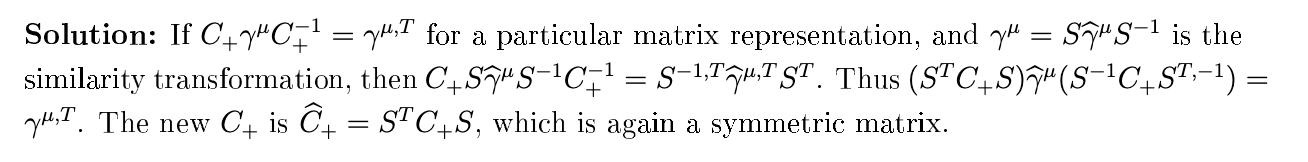
\includegraphics[width=\textwidth]{Figures/pvnsolution.png}
\end{figure}


\subsubsection{Normal modes of atoms}

Molecules with multiple atoms generally obey
a periodic structure, and thus they are symmetric
under certain operations (translations and rotations).
Generally, symmetry constrains dynamics, and it is no diff
here: we can decompose a molecule's normal modes through
group theory, specifically through decomposing the characters
of reducible representations into irreps, thus giving us \note{multiplets?
or smth like that. idk.}

Let us define a few things first. A molecule with $N$ atoms
can be described by the $3N$-dimensional vector $\mathbf{X} = (\bfx_1, \ldots, \bfx_N)$.
Considering deviations from equilibrium for each atom
and defining $\boldsymbol{\xi}_a = \bfx_a - \bfx_a^0$
gives $\widetilde{\mathbf{X}} = (\boldsymbol{\xi}_1, \ldots, \boldsymbol{\xi}_N)$.
The energy associated with the small deviations of the molecule is
then
\begin{align*}
    H = \frac{1}{2}m_\alpha (\partial_t \widetilde{X}_\alpha)^2 + \frac{1}{2}K_{\alpha \beta} \widetilde{X}_\alpha \widetilde{X}_\beta.
\end{align*}
where $\alpha, \beta = 1, \ldots, 3N$. We may rescale 
$\boldsymbol{\xi}_a \to \boldsymbol{\xi}_a/\sqrt{m_a} = \boldsymbol{\lambda}_a$,
and then orthogonalize $K_{\alpha \beta}'$ as it's symmetric;
we then have the equation \note{PvN's equation is wrong with
index contractions, fix later}


There are three ingredients we need to consider
to represent our atom using representation theory:
\begin{itemize}
    \item We need \textbf{two} representations. One of them
    is a permutation representation, $A \colon G \to \Aut(V)$,
    and the other is a rotation representation, $R \colon G \to D_n \subset SO(3)$.
    \item We need \textbf{one} group action, $\pi \colon G \times G \to G$,
    which acts to permute the labels of our atoms, $s$.
\end{itemize}

We then need to consider the characters of these representations,
and we need to find out how many irreps are contained within them.
The use of the group action is that it just lets our representations 
talk to each other via projections through the following equation:
\begin{align*}
    \boxed{\mathcal{P}_{\pi_s} A_g \widetilde{\mathbf{X}} = D(g) \mathcal{P}_s \widetilde{\mathbf{X}}.}
\end{align*}
In words, this tells you that permuting atoms and rotating them
is the same thing\footnote{PvN remarked upon this multiple times
while showing us the demonstration that ``To half of you this will
be incredibly obvious, and half of you will not understand
this no matter how many times I say it. Now you know if you're
a physicist or a mathematician, no one told you before but now you know.''
\note{fix quote}}.

Consider the character for rotations, $\chi_{\reals^3}$. This is related
to the genuine normal modes by
\begin{align*}
    \boxed{\chi_{\rm gen} = \chi_S - \chi_{\rm tr} - \chi_{\rm rot} = \chi_{\reals^3} (c_g - 1 - \det{D}),}
\end{align*}
so $\chi_S = c_g \chi_{\reals^3}$, $\chi_{\rm tr} = \chi_{\reals^3}$,
taking all of the possible modes and subtracting out the trivial ones.
It is only slightly reductionistic to say that this is the most important equation
in this entire analysis. Our entire goal will be to find $\chi_{\rm gen}$
and then take inner products of it with our irrep characters to find how 
many irreps are contained in the genuine motion.

\note{explain why the relations between the rotations and the other
trivial modes are true}

The general process for determining the normal modes of a molecule
goes as follows:
\begin{enumerate}
    \item Analyze the number of normal modes using the formulae
    $n = 2N - 3$, $n = 3N - 6$. \note{check formula for d = 2}
    \item Determine the symmetry group of the molecule.
    \item Find the classes of the group and their orders.
    \item Find the commutator subgroup of the group.
    \item Find the dimensions of the irreps.
    \item Find the character table for the irreps
    \item Find $\chi_{\rm tr}$, $\chi_{\rm rot}$, and $\chi_S$
    through $\chi_{\reals^3}$.
    \item Find $\chi_{\rm gen}$.
    \item Take inner products of the normal modes to determine
    the decomposition of $\chi_{\rm gen}$.
    \item Write the motion as a direct sum of irreps.
    \item Using symmetry considerations, determine the
    physical realization of the normal modes.
\end{enumerate}

We now show a number of canonical examples, answering the standard
questions for each molecule.

\begin{eexample}
    [Triangle]
    We have:
    \begin{enumerate}
        \item The symmetry group is $D_3$.
        \item The classes are $\{ e \}$, $\{ (12) \}$, $\{ (123) \}$.
        Their orders are $1 + 3 + 2 = 6$.
        \item The commutator subgroup is $A_3$.
        \item There are $2$ $1D$-irreps and $1$ $2D$-irrep.
        \item The character table is
        \begin{table}[H]
            \centering
            \begin{tabular}{|c|c|c|c|c|c|}
                \hline
                 & $e$ & $(12)$ & $(123)$\\
                 & $1$ & $3$ & $2$\\
                \hline
                $\id$ & $1$ & $3$ & $2$\\
                ${\rm sgn}$ & $1$ & $-1$ & $1$\\
                $\chi^2$ & $2$ & $0$ & $-1$\\
                $\chi_{\rm gen}$ & $2$ & $0$ & $2$\\
                \hline
            \end{tabular}
        \end{table}
        \item We can use the formula $\chi_{\rm gen} = \chi^2 (c_g - 1 - \det{D})$,
        to get the last row of the table above.
        \item Taking inner products gives
        \begin{align*}
            (\chi_{\rm gen}, \id) & = \frac{1}{6} (2 + 4) = 1,\\
            (\chi_{\rm gen}, \sgn) & = \frac{1}{6} (2 + 4) = 1,\\
            (\chi_{\rm gen}, \chi^2) & = \frac{1}{6} (4 - 4) = 0.
        \end{align*}
        \item So our motion is
        \begin{align*}
            \boxed{\Omega = A_1 \oplus A_2.}
        \end{align*}
        \item This corresponds to the breather and the stretcher.
    \end{enumerate}
\end{eexample}


\begin{eexample}
    [Square]
    We have:
    \begin{enumerate}
        \item There are $2N - 3 = 5$ non-trivial planar normal modes,
        and $3N - 6 = 6$ non-trivial 3D normal modes.
        \item The symmetry group is $D_4$.
        \item The classes are $\{ e \}$, $\{ r, r^3 \}$, $\{ r^2 \}$, $\{ \sigma r, \sigma r^3 \}$, $\{ \sigma, \sigma r^2 \}$.
        Their orders are obvious.
        \item The commutator subgroup is $\{e, r^2 \}$.
        \item There are $4$ $1D$-irreps and there is $1$ $2D$-irrep.
        \item The character table is
        \begin{table}[H]
            \centering 
            \begin{tabular}{|c|c|c|c|c|c|}
                \hline
                & $e$ & $r^2$ & $r^{2k + 1}$ & $\sigma r^2$ & $\sigma r^{2k + 1}$\\
                & $1$ & $1$ & $2$ & $2$ & $2$\\
                \hline
                $\id$ & $1$ & $1$ & $1$ & $1$ & $1$\\
                $\sgn$ & $1$ & $1$ & $-1$ & $1$ & $-1$\\
                $\chi^1$ & $1$ & $1$ & $-1$ & $1$ & $-1$\\
                $\chi^2$ & $1$ & $1$ & $-1$ & $-1$ & $1$\\
                $\chi_{2D}$ & $2$ & $-2$ & $0$ & $0$ & $0$\\
                $\chi_{\rm gen}$ & $4$ & $4$ & $0$ & $0$ & $0$\\
                \hline
            \end{tabular}
        \end{table}
        \item See above, use $\chi_{\rm gen} = \chi_{2D}(c_g - 1 - \det{D})$.
        \item Taking inner products gives
        \begin{align*}
            (\chi_{\rm gen}, \id) & = \frac{1}{8} (4 + 4) = 1,\\
            (\chi_{\rm gen}, \sgn) & = \frac{1}{8} (4 + 4) = 1,\\
            (\chi_{\rm gen}, \chi^1) & = \frac{1}{8} (4 + 4) = 1,\\
            (\chi_{\rm gen}, \chi^2) & = \frac{1}{8} (4 + 4) = 1,\\
            (\chi_{\rm gen}, \chi_{2D}) & = \frac{1}{8} (8 - 8) = 0.
        \end{align*}
        \item So our motion is
        \begin{align*}
            \boxed{\Omega = A_1 \oplus A_2 \oplus A_3 \oplus A_4.}
        \end{align*}
        \item This corresponds to the breather, the (out-of-plane) twister, 
        the (x-y) stretcher, and the (diagonal) shearer.
    \end{enumerate}
\end{eexample}

\begin{eexample}
    [Tetrahedron]
    We have:
    \begin{enumerate}
        \item The symmetry group is $S_4$.
        \item The classes are $\{ e \}$, $\{ (12) \}$, $\{ (123) \}$, $\{ (12)(34)\}$, and $\{ (1234) \}$.
        Their orders are $1 + 6 + 6 + 3 + 8 = 24$.
        \item The commutator subgroup is $A_4$.
        \item There are $2$ $1D$-irreps, $1$ $2D$-irrep, and $2$ $3D$-irreps.
        \item The character table is
        \begin{table}[H]
            \centering
            \begin{tabular}{|c|c|c|c|c|c|}
                \hline
                 & $e$ & $(12)$ & $(123)$ & $(12)(34)$ & $(1234)$\\
                 & $1$ & $6$ & $6$ & $3$ & $8$\\
                \hline
                $\id$ & $1$ & $1$ & $1$ & $1$ & $1$\\
                $\operatorname{sgn}$ & $1$ & $-1$ & $1$ & $1$ & $-1$\\
                $\chi^2$ & $2$ & $0$ & $-1$ & $2$ & $0$\\
                $\chi^3$ & $3$ & $1$ & $0$ & $-1$ & $-1$\\    
                $\chi^3_{\rm sgn}$ & $3$ & $-1$ & $0$ & $-1$ & $1$\\
                $\chi_{\rm gen}$ & $6$ & $2$ & $0$ & $2$ & $0$\\
                \hline
            \end{tabular}
        \end{table}
        Some explanation for the table:
        \begin{itemize}
            \item Identity and sign are obvious.
            \item $\chi^2$ is difficult to find. You get it through orthogonality
            with the other rows, as there are four equations and four unknowns.
            \item $\chi^3$ is given through finding $1 + 2\cos{\theta}$ for each
            entry, with $1$ for reflections.
            \item $\chi^3_{\rm sgn}$ is $\chi^3 \, {\rm sgn}$.
        \end{itemize}
        \item We can use the formula $\chi_{\rm gen} = \chi^3 (c_g - 1 - \det{D})$
        to fill in the last row of the table, as given above.
        \item Taking inner products, we have
        \begin{align*}
            (\chi_{\rm gen}, \chi^2) & = \frac{1}{24} (6 + 12 + 0 + 6 + 0) = 1,\\
            (\chi_{\rm gen}, \chi^2) & = \frac{1}{24} (12 + 0 + 0 + 12 + 0) = 1,\\
            (\chi_{\rm gen}, \chi^3) & = \frac{1}{24} (18 + 12 + 0 - 6 + 0) = 1,\\
            (\chi_{\rm gen}, \chi^3_{\rm sgn}) & = \frac{1}{24} (18 - 12 + 0 - 6 + 0) = 0.
        \end{align*}
        \item Thus, our motion is
        \begin{align*}
            \boxed{\Omega = A_1 \oplus A_2 \oplus A_3.}
        \end{align*}
        \item Physically, $A_1$ is the breather, $A_2$ is the four
        pumpers (along and against a line), and $A_3$ is the three twisters (twisting any
        two edges in the opposite way).
    \end{enumerate}
\end{eexample}

\begin{eexample}
    [Triangle with dot]
\end{eexample}

\begin{eexample}
    [Square with dot]
\end{eexample}

\begin{eexample}
    [Tetrahedron with dot]
\end{eexample}

\note{don't really need to add any examples 
that PvN already has in his notes}

\note{add other common examples}

\end{document}